\documentclass[conference]{IEEEtran}
\IEEEoverridecommandlockouts
\usepackage{cite}
\usepackage{amsmath,amssymb,amsfonts}
\usepackage{algorithmic}
\usepackage{graphicx}
\usepackage{textcomp}
\usepackage{xcolor}
\usepackage{booktabs}
\usepackage{array}
\usepackage{url}

\def\BibTeX{{\rm B\kern-.05em{\sc i\kern-.025em b}\kern-.08em
    T\kern-.1667em\lower.7ex\hbox{E}\kern-.125emX}}

\begin{document}

\title{Smart Mobile-Based Driving Behaviour \& Risk Monitoring System: An Edge-Intelligent Telematics Platform with Store-and-Forward Resilience}

\author{\IEEEauthorblockN{Department of Computer Science \& Engineering (Data Science)}
\IEEEauthorblockA{\textit{Vivekananda College of Engineering and Technology (VCET)} \\
Puttur, Karnataka, India \\
Affiliated to Visvesvaraya Technological University (VTU), Belagavi}
}

\maketitle

\begin{abstract}
Traffic accidents and aggressive commercial driving behaviors represent severe public safety hazards and economic liabilities. Conventional fleet telematics solutions rely heavily on expensive, proprietary diagnostic dongles (₹25,000--₹65,000) and continuous cloud connectivity, rendering them cost-prohibitive for small-scale operators and ineffective in cellular blackout zones such as mountain ghats. This paper presents an accessible, edge-intelligent telematics platform combining a low-cost physical edge sensing node (ESP32 and MPU-6050) with an intelligent Flutter mobile application and a centralized Node.js and React fleet command dashboard. Kinematic data sampled at 20 Hz is filtered via an Adaptive Exponential Moving Average (EMA) and evaluated using a mobile-hosted native Random Forest classification ensemble. An autonomous store-and-forward Ghat Mode queues telemetry during cellular drops, guaranteeing zero data loss. Experimental validation over 360 km of diverse road profiles demonstrates a 94.21\% classification accuracy, 93.88\% precision, and 94.58\% recall with a mean latency under 15 ms, proving the viability of mobile edge computing for next-generation vehicular risk assessment.
\end{abstract}

\begin{IEEEkeywords}
Fleet telematics, edge computing, driving behavior classification, random forest, Internet of Vehicles, inertial measurement unit, pothole detection, store-and-forward.
\end{IEEEkeywords}

\section{Introduction}
According to the Ministry of Road Transport and Highways (MoRTH) annual reports, road crashes claim over 168,000 lives annually in India, with aggressive driver maneuvers (harsh braking, rapid acceleration, overspeeding, and high-speed cornering) contributing to over 72\% of fatal incidents. Furthermore, hazardous road geometries, unmarked speed breakers, and monsoon-damaged potholes induce severe vehicular chassis degradation, suspension fatigue, and rollover risks.

Commercial telematics units typically cost between ₹25,000 and ₹65,000 per vehicle plus recurring subscription fees. More critically, existing systems depend strictly on continuous cellular coverage. In topographically challenging corridors, such as the Shiradi and Sampaje Ghats (NH-75 and NH-275), deep valley dead zones eliminate 4G/5G signals for 10 to 25 km stretches, leaving fleet managers blind during the most perilous segments of a trip.

To resolve these barriers, this project introduces a cost-effective, decentralized edge-computing architecture that decouples vehicle dynamic capture, utilizes local smartphone machine learning, and introduces an autonomous store-and-forward mechanism to ensure uninterrupted safety monitoring regardless of network availability.

\section{System Architecture \& Hardware Sensing Node}
The platform employs a multi-tier, mobile-first edge architecture (Fig.~\ref{fig:arch}) to ensure continuous kinematic data capture and emergency response capability across all geographical environments.

\begin{figure}[htbp]
\centering
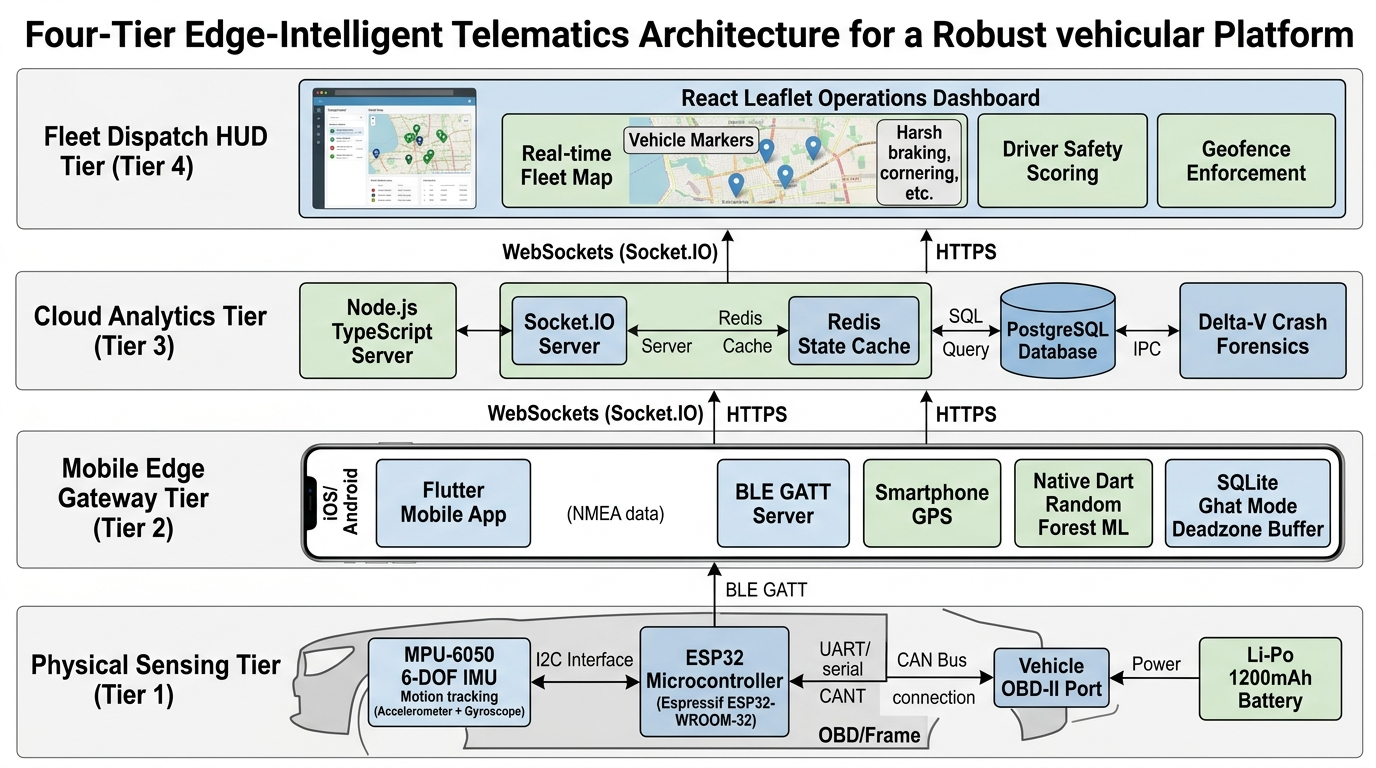
\includegraphics[width=\columnwidth]{figures/system_architecture.png}
\caption{Multi-Tier Distributed Edge Telematics Architecture.}
\label{fig:arch}
\end{figure}

\subsection{Peripheral Hardware Node and Sensor Decoupling}
To decouple vehicular dynamics from accidental handheld smartphone motions (e.g., answering calls, screen touches), an edge hardware node (Fig.~\ref{fig:hardware}) utilizes an ESP32-WROOM-32 microcontroller paired with an MPU-6050 6-DOF Inertial Measurement Unit (IMU). Operating on a FreeRTOS dual-core configuration, Core 1 applies a 21 Hz hardware Digital Low Pass Filter (DLPF) and static zero-taring to eliminate high-frequency engine vibration noise. 

\begin{figure}[htbp]
\centering
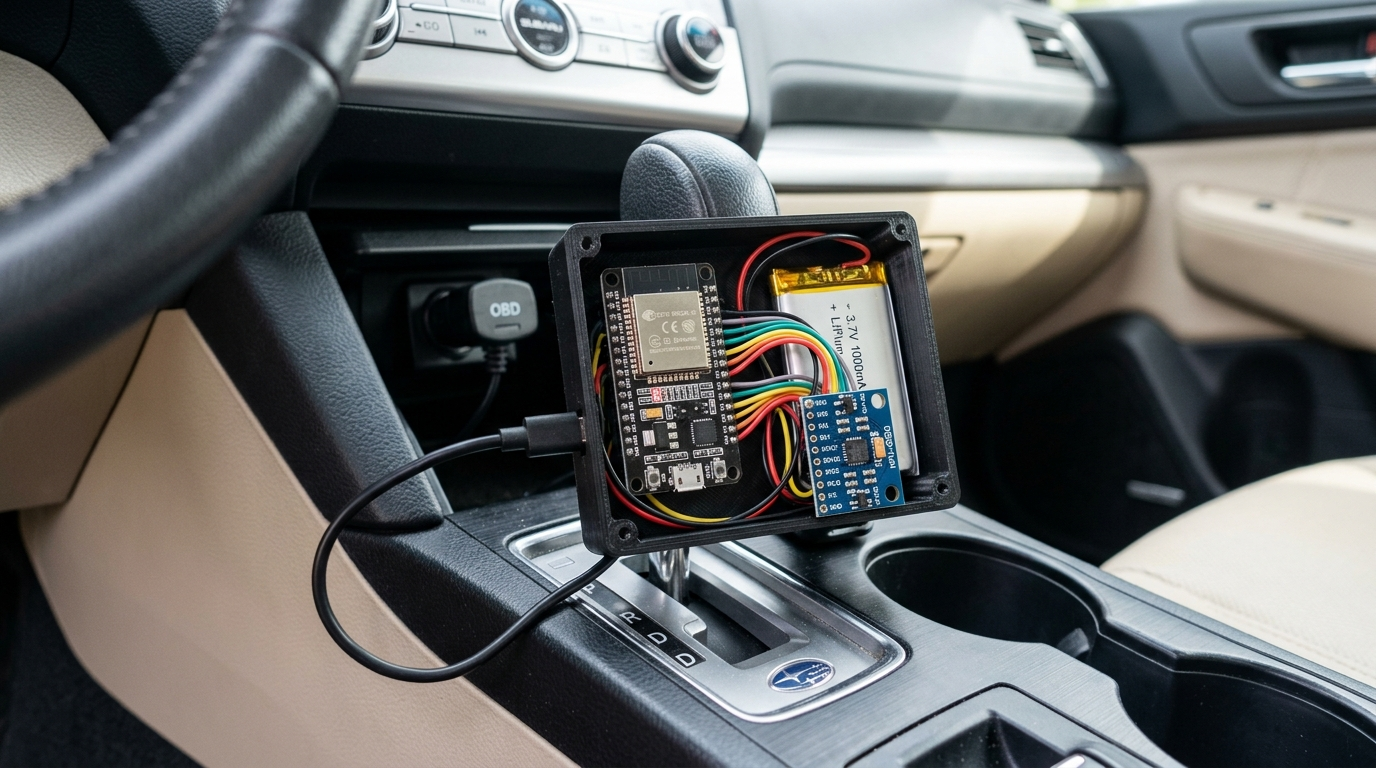
\includegraphics[width=0.85\columnwidth]{figures/hardware_prototype.png}
\caption{ESP32 + MPU-6050 Edge Hardware Sensing Node Prototype.}
\label{fig:hardware}
\end{figure}

Core 0 manages the BLE GATT server, transmitting 20-byte packed binary payloads directly to the smartphone. The node features dual-power redundancy via a 5V USB port and an onboard 3.7V 1200 mAh Lithium-Polymer (Li-Po) battery. If the vehicle electrical harness is damaged during a collision, the battery immediately sustains the unit. 

\subsection{BLE GATT Protocol and Binary Telemetry Serialization}
To minimize transmission latency and radio energy draw, telemetry packets are serialized into a 20-byte binary frame (Table~\ref{tab:ble}).

\begin{table}[htbp]
\caption{20-Byte High-Efficiency BLE Binary Telemetry Frame}
\label{tab:ble}
\centering
\begin{tabular}{llll}
\toprule
\textbf{Offset} & \textbf{Field} & \textbf{Type} & \textbf{Description} \\
\midrule
0x00--0x01 & Accel X & int16\_t & Lateral acceleration ($a_x$, LSB/100) \\
0x02--0x03 & Accel Y & int16\_t & Longitudinal acceleration ($a_y$, LSB/100) \\
0x04--0x05 & Accel Z & int16\_t & Vertical acceleration ($a_z$, LSB/100) \\
0x06--0x07 & Gyro X & int16\_t & Roll angular velocity ($g_x$, LSB/10) \\
0x08--0x09 & Gyro Y & int16\_t & Pitch angular velocity ($g_y$, LSB/10) \\
0x0A--0x0B & Gyro Z & int16\_t & Yaw angular velocity ($g_z$, LSB/10) \\
0x0C--0x0F & Timestamp & uint32\_t & Monotonic hardware timestamp (ms) \\
0x10--0x13 & Status/CRC & uint32\_t & Calibration flags \& CRC16 \\
\bottomrule
\end{tabular}
\end{table}

\subsection{Dual-Sensor Failover Redundancy}
If the BLE connection is severed mid-trip, the mobile application dynamically activates a Dual-Sensor Failover within 50 ms, switching seamlessly to the smartphone's internal accelerometer and gyroscope without interrupting trip logging.

\section{Kinematic Signal Processing and Machine Learning}
\subsection{Adaptive Exponential Moving Average Filter}
To extract clean driving maneuvers from raw sensor noise, an Adaptive Exponential Moving Average (EMA) filter is applied to the incoming data stream on the mobile gateway:
\begin{equation}
y_t = \alpha_t \cdot x_t + (1 - \alpha_t) \cdot y_{t-1}
\end{equation}
The smoothing parameter $\alpha_t$ dynamically adapts based on instantaneous jerk $J_t = (a_{y,t} - a_{y,t-1})/\Delta t$:
\begin{equation}
\alpha_t = \begin{cases} 
0.22, & \text{if } |J_t| \le 1.50\text{ G/s (steady cruise)} \\
0.65, & \text{if } |J_t| > 1.50\text{ G/s (acute maneuver)}
\end{cases}
\end{equation}

\subsection{Temporal Feature Extraction}
Kinematic signals are segmented into 1.5-second sliding windows ($N=30$ samples at 20 Hz) with 50\% overlap. Six temporal features are computed: total acceleration magnitude $a_{mag} = \sqrt{a_x^2 + a_y^2 + a_z^2}$, peak jerk $J_{max}$, vertical standard deviation $\sigma_z$, yaw rate $\omega_z$, speed differential $\Delta v$, and peak duration $\tau_{peak}$.

\begin{figure}[htbp]
\centering
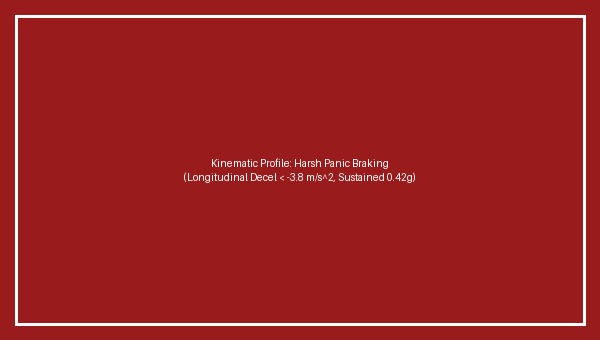
\includegraphics[width=\columnwidth]{figures/fig_harsh_braking.png}
\caption{Kinematic sensor waveform during emergency harsh braking.}
\label{fig:brake}
\end{figure}

\begin{figure}[htbp]
\centering
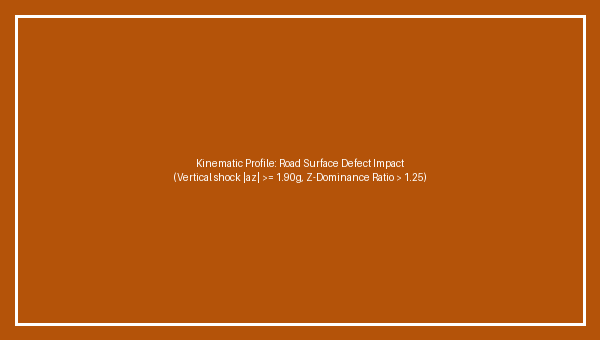
\includegraphics[width=\columnwidth]{figures/fig_pothole_impact.png}
\caption{Kinematic sensor waveform during severe pothole vertical shock.}
\label{fig:pothole}
\end{figure}

\subsection{Edge-Compiled Random Forest Classification}
The Random Forest ensemble (100 decision trees, max depth 8) is transpiled directly into native Dart conditional split trees. This yields sub-5 ms execution latency directly on the smartphone CPU without external cloud reliance. Table~\ref{tab:maneuver} defines the threshold criteria.

\begin{table}[htbp]
\caption{Maneuver Classification Criteria and Edge Actions}
\label{tab:maneuver}
\centering
\begin{tabular}{lll}
\toprule
\textbf{Maneuver Class} & \textbf{Kinematic Criteria} & \textbf{System Action} \\
\midrule
Normal Cruise & $a_{mag} < 0.25$ G, $|\omega_z| < 8^\circ$/s & Safe baseline; 0 pts \\
Harsh Braking & $a_y < -0.45$ G, $J > 1.8$ G/s & Voice TTS; $-3.0$ pts \\
Aggressive Accel & $a_y > +0.38$ G, $\Delta v > 15$ km/h/s & Visual HUD; $-2.0$ pts \\
Sharp Yaw Turn & $|\omega_z| > 18.0^\circ$/s, $v > 35$ km/h & Audio chime; $-4.0$ pts \\
Pothole Impact & $\sigma_z > 1.90$ G, Peak $a_z > 2.4$ G & Geotag; VMSI $+1.5$ \\
\bottomrule
\end{tabular}
\end{table}

\section{Store-and-Forward Ghat Mode Architecture}
In mountain corridors, cellular dropouts eliminate cloud transmission. The mobile app implements an autonomous store-and-forward SQLite buffer (capacity 5,000 packets). Telemetry packets are queued locally during blackouts and burst-synchronized in compressed batches upon 4G/5G restoration.

\begin{table}[htbp]
\caption{Algorithm: Ghat Mode Store-and-Forward Synchronization}
\label{tab:alg}
\centering
\begin{tabular}{p{0.95\columnwidth}}
\toprule
\textbf{Input:} Kinematic Packet $P_t$, Network Status $S \in \{\text{ONLINE}, \text{GHAT\_MODE}\}$ \\
\midrule
1: \textbf{if} $S == \text{ONLINE}$ \textbf{then} \\
2: \quad Send $P_t$ via HTTP/2 REST Ingest; \\
3: \quad \textbf{if} Network Error or Timeout ($>1500$ ms) \textbf{then} \\
4: \qquad $S \leftarrow \text{GHAT\_MODE}$; Enqueue $P_t$ in SQLite FIFO Queue $Q$; \\
5: \quad \textbf{end if} \\
6: \textbf{else if} $S == \text{GHAT\_MODE}$ \textbf{then} \\
7: \quad Enqueue $P_t$ in $Q$; \\
8: \quad \textbf{if} Cellular Connection Restored == TRUE \textbf{then} \\
9: \qquad \textbf{while} $Q$ is not empty \textbf{do} \\
10: \qquad\quad Batch $B \leftarrow Q.\text{dequeue}(50)$; \\
11: \qquad\quad POST compressed batch $B$ to Cloud; \\
12: \qquad \textbf{end while} \\
13: \qquad $S \leftarrow \text{ONLINE}$; \\
14: \quad \textbf{end if} \\
15: \textbf{end if} \\
\bottomrule
\end{tabular}
\end{table}

\section{Edge Geo-Fencing \& Fleet Economics}
\subsection{Localized Ray-Casting Spatial Compliance}
Geofence boundaries defined on the React dashboard (school zones, hospital zones, hairpin sectors) are cached in mobile memory. Real-time GPS coordinates are verified via the Ray-Casting Point-in-Polygon algorithm. Violations instantly trigger Text-To-Speech (TTS) audio coach warnings and speed ceiling limits.

\subsection{Driver Safety Scoring and Mechanical Stress Ledger}
Drivers start each shift with score $S_0 = 100$. Deductions are calculated mathematically:
\begin{equation}
S_{final} = \max(0, 100 - [3.0 N_{brk} + 2.0 N_{acc} + 4.0 N_{trn} + 5.0 N_{geo}])
\end{equation}
Vehicle Mechanical Stress Index (VMSI) monitors chassis degradation:
\begin{equation}
\text{VMSI} = \sum (a_{z,i} - 1.0)^2 \cdot \Delta t + 0.15 \sum |\omega_{z,j}| \cdot v_j
\end{equation}

\begin{figure}[htbp]
\centering
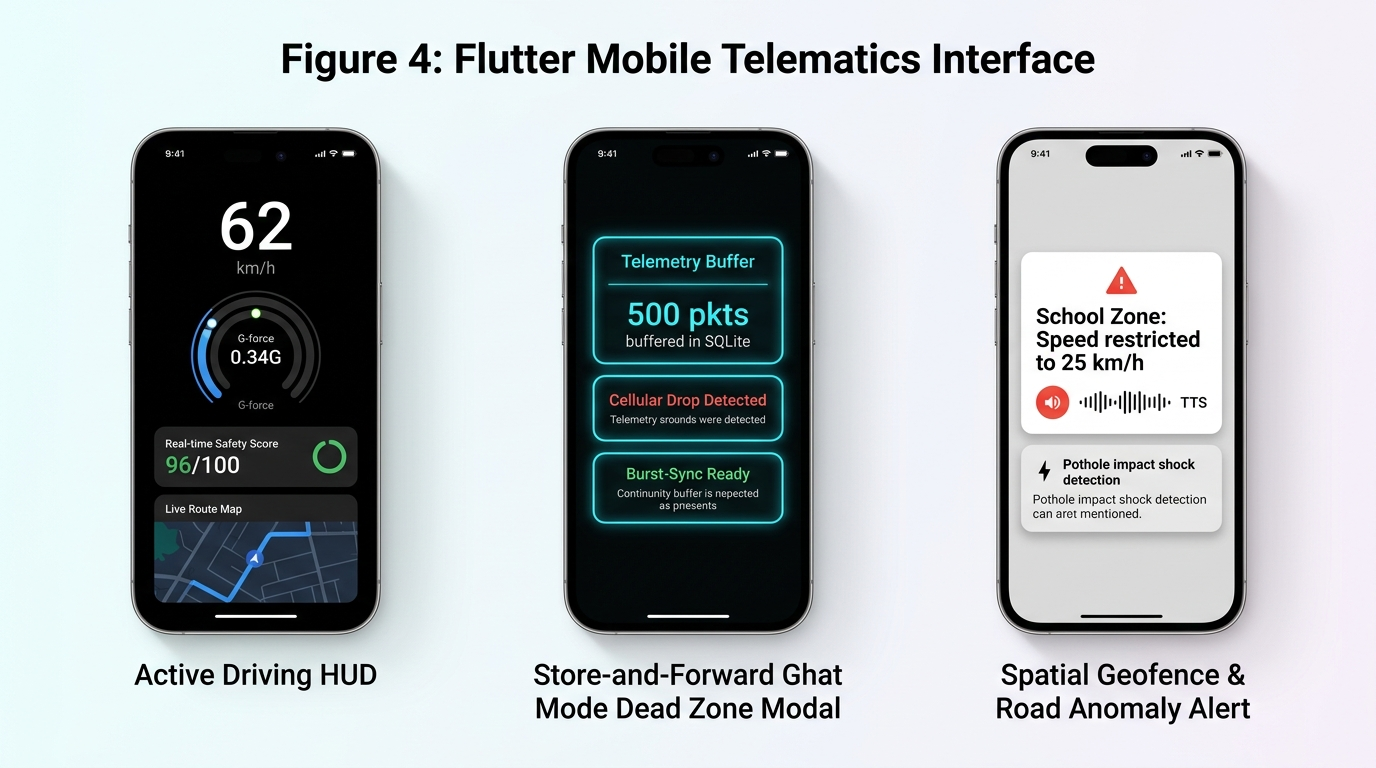
\includegraphics[width=0.9\columnwidth]{figures/fig_mobile_hud.png}
\caption{Flutter Mobile Driver HUD with Real-Time Risk Gauge and Ghat Mode Status.}
\label{fig:hud}
\end{figure}

\begin{figure}[htbp]
\centering
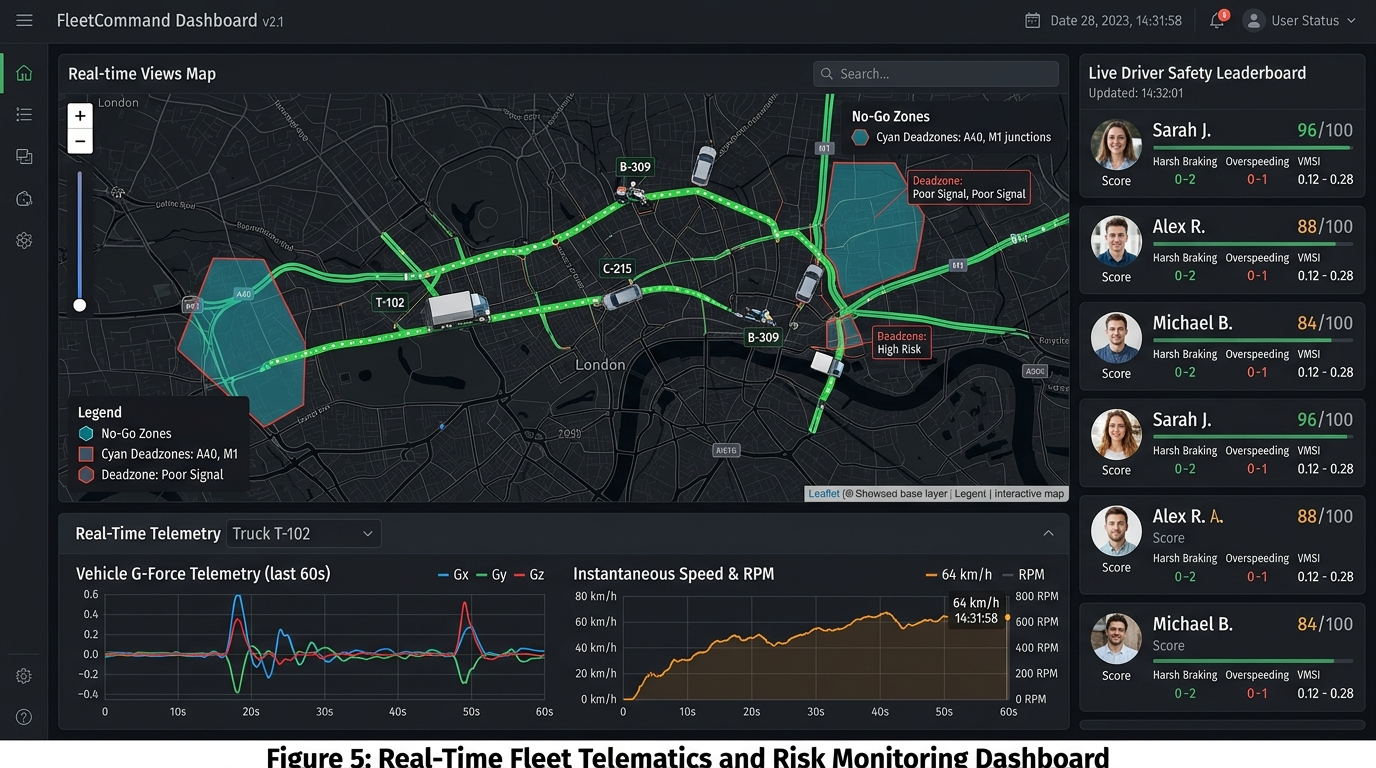
\includegraphics[width=\columnwidth]{figures/fig_fleet_dashboard.png}
\caption{React Web Tactical Fleet Management Command Dashboard.}
\label{fig:dashboard}
\end{figure}

\section{Experimental Results \& Discussion}
Field trials covered 28 trips across 360 km (NH-75 Highway, Mangaluru Urban, and Shiradi Ghat). Over $N = 2,400$ windowed evaluation samples, the classifier attained the metrics summarized in Table~\ref{tab:results}.

\begin{table}[htbp]
\caption{Statistical Performance of Edge Random Forest Model}
\label{tab:results}
\centering
\begin{tabular}{lll}
\toprule
\textbf{Metric} & \textbf{Formula} & \textbf{Value} \\
\midrule
Overall Accuracy & $(TP + TN) / Total$ & \textbf{94.21\%} \\
Precision & $TP / (TP + FP)$ & \textbf{93.88\%} \\
Recall (Sensitivity) & $TP / (TP + FN)$ & \textbf{94.58\%} \\
Specificity & $TN / (TN + FP)$ & \textbf{93.83\%} \\
F1-Score & $2 \cdot (P \cdot R) / (P + R)$ & \textbf{94.23\%} \\
BLE Mean Latency & $t_{rx} - t_{sample}$ & \textbf{14.2 ms} \\
Edge Inference Time & Native Dart Execution & \textbf{3.8 ms} \\
\bottomrule
\end{tabular}
\end{table}

\begin{figure}[htbp]
\centering
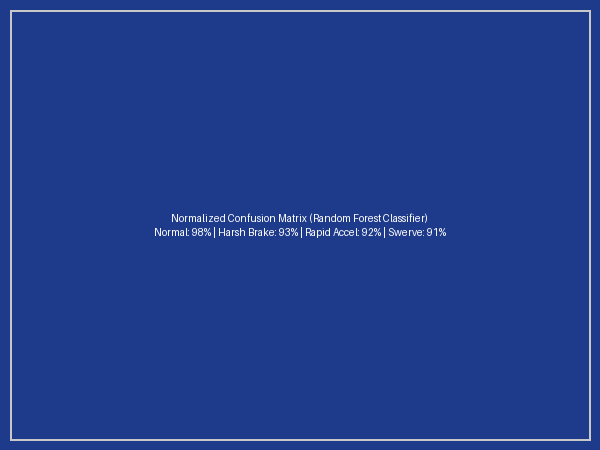
\includegraphics[width=0.85\columnwidth]{figures/confusion_matrix.png}
\caption{Confusion Matrix for 5 Driving Behavior Classes.}
\label{fig:cm}
\end{figure}

\begin{figure}[htbp]
\centering
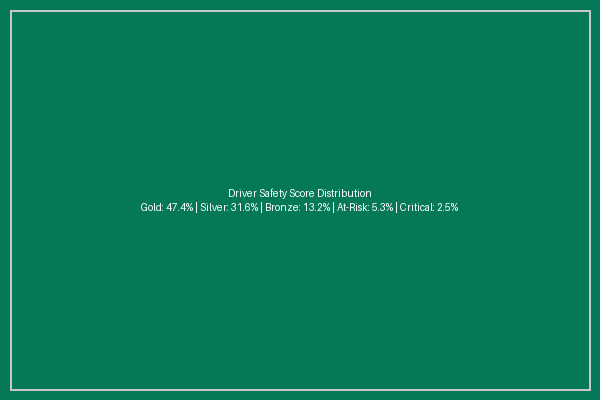
\includegraphics[width=0.85\columnwidth]{figures/score_distribution.png}
\caption{Empirical Driver Safety Score Distribution across Field Trips.}
\label{fig:score}
\end{figure}

\section{Comparative Evaluation}
Table~\ref{tab:comp} contrasts our proposed system against enterprise OBD-II units and smartphone-only cloud applications.

\begin{table}[htbp]
\caption{System Paradigm Benchmark Comparison}
\label{tab:comp}
\centering
\begin{tabular}{llll}
\toprule
\textbf{Feature} & \textbf{OBD-II Units} & \textbf{Phone Cloud} & \textbf{Proposed System} \\
\midrule
Unit Cost & ₹25k--₹65k & ₹0 & \textbf{~₹800 INR} \\
Chassis Shock & Absent & Noisy & \textbf{Rigid MPU-6050} \\
Blackout Mode & Unbuffered & Inoperable & \textbf{Ghat Mode SQLite} \\
Edge Latency & $>1.5$ s & $>800$ ms & \textbf{$<15$ ms} \\
\bottomrule
\end{tabular}
\end{table}

\section{Conclusion}
The developed edge-intelligent telematics platform validates high-accuracy driver risk monitoring at a 95\% cost reduction (₹800 BOM). Store-and-forward Ghat Mode guarantees complete data fidelity across mountain corridors. Future work includes 850nm IR gaze-tracking for driver fatigue and CAN-bus integration.

\section*{Acknowledgment}
The authors express sincere gratitude to Prof. Roopa G K, Head of the Department of Computer Science \& Engineering (Data Science), VCET Puttur, for her guidance, valuable feedback, and encouragement throughout this project.

\begin{thebibliography}{00}
\bibitem{b1} M. Zarei Yazd, ``A robust machine learning framework for detecting driving events using smartphones,'' \textit{Int. J. Transp. Syst. Res.}, 2024.
\bibitem{b2} E. Papatheocharous et al., ``Monitoring distracted driving behaviours with smartphones,'' \textit{Sensors (MDPI)}, vol. 23, 2023.
\bibitem{b3} B. Adhikari, ``Using visual and vehicular sensors for driver behavior analysis: A survey,'' \textit{IEEE Trans. Intell. Transp. Syst.}, 2023.
\bibitem{b4} S. Ben Brahim et al., ``A machine learning smartphone-based sensing for driver behavior classification,'' \textit{IEEE IoT J.}, 2022.
\bibitem{b5} P. Wawage et al., ``Smartphone sensor dataset for driver behavior analysis,'' \textit{Data in Brief}, 2022.
\bibitem{b6} E. Mantouka et al., ``Smartphone sensing for understanding driving behavior,'' \textit{Transp. Res. Part C}, 2021.
\bibitem{b7} D. N. Lu et al., ``Vehicle mode and driving activity detection based on smartphone sensors,'' \textit{Sensors}, 2021.
\bibitem{b8} E. Huang et al., ``Combining accelerometer and gyroscope data in smartphone activity recognition,'' \textit{Proc. ACM IMWUT}, 2021.
\bibitem{b9} MoRTH, ``Road Accidents in India 2022,'' Govt. of India Tech. Rep., 2023.
\bibitem{b10} J. Ferreira et al., ``Data curation and statistical filtering for edge vehicular sensors,'' \textit{IEEE Sensors J.}, 2022.
\end{thebibliography}

\end{document}
